\def\QRCODE{MASTER_mispa_TUT.IMG.lip_matlabqrcode.png}
\def\QRPAGE{http://www.iptutorials.science/tree/master/MASTER_mispa/TUT.IMG.lip/matlab}
\mcorrectionsection{Matlab correction}
\subsection{Elementary operations}
The most important function to code is the \lstinline!graytone! transformation function. It considers $M$ as the maximum value (the absolute white). This code means that the absolute white cannot be reached, and thus $f\in[0;M[$. After discretizing the gray values, $F\in[0;M-1]$.

\begin{matlab}
function f=graytone(F, M)
% graytone transform
% this is the most important
f = M-eps(M)-F;
\end{matlab}

\begin{matlab}
function l=phi(f, M)
% isomorphism
l = -M*log(1-f/M);
end

function f=invphi(l)
f = M*(1-exp(-l/M));
end
\end{matlab}


\begin{matlab}
function z=plusLIP(x,y,M)
a=double(x);
b=double(y);
z=a+b-a.*b/M;
\end{matlab}

\begin{matlab}
function z=timesLIP(alpha,x,M)
a=double(x);
z=M-M*(1-a/M).^alpha;
\end{matlab}

\subsection{LIP dynamic expansion}
The optimal value for dynamic expansion is given by $\lambda_0$:
$$\lambda_0(f)=\arg\max_{\lambda}\left\{\max(\lambda\lipfois{} f)-\min(\lambda\lipfois{} f) \right\}$$

Let $A(\lambda)=\max(\lambda\lipfois{} f)-\min(\lambda\lipfois{} f)=\lambda\lipfois{}\max(f)-\lambda\lipfois{}\min(f)$ and $B=\ln(1-\min(f)/M)$ et $C=\ln(1-\max(f)/M)$.


\begin{eqnarray*}
A'(\lambda)=0&\Leftarrow &[(M-M\exp(\lambda C))-(M-M\exp(\lambda B))]'=0\\
&\Leftarrow & [\exp(\lambda B)-\exp(\lambda C)]'=0\\
&\Leftarrow & B\exp(\lambda B)-C\exp(\lambda C)=0\\
&\Leftarrow & \ln(B)+\lambda B=\ln(C) -\lambda C\\
&\Leftarrow & \lambda=\frac{\ln(C)-\ln(B)}{B-C}\\
&\Leftarrow & \lambda=\frac{\ln(C/B)}{B-C}
\end{eqnarray*}
Thus, yielding to:
$$\lambda_0(f)=\frac{\displaystyle\ln\left(\frac{\ln(1-\max(f)/M)}{\ln(1-\min(f)/M)}\right)}{\displaystyle\ln\left(\frac{M-\min(f)}{M-\max(f)}\right)}$$

The results are shown in Fig. \ref{fig:lip:results}.
\begin{figure}[htbp]
 \centering
 \subfloat[Original image.]{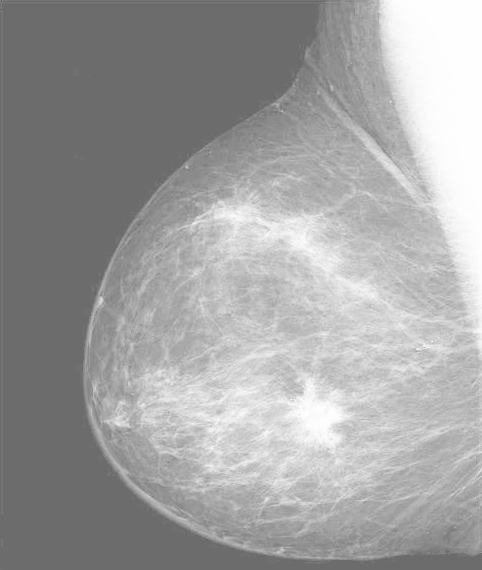
\includegraphics[width=5cm]{breast.png}}\hspace{.5cm}
 \subfloat[LIP dynamic expansion.]{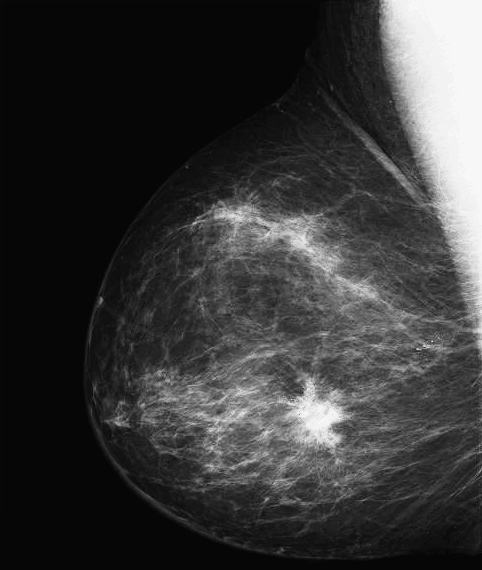
\includegraphics[width=5cm]{expanded.png}}\hspace{.5cm}
 \subfloat[Histogram equalization.]{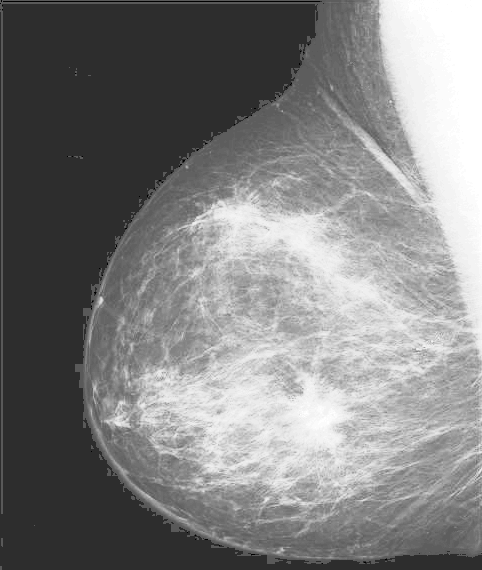
\includegraphics[width=5cm]{histeq.png}}
 \caption{Results of dynamic expansion. The dark part of the image appears darker.} \label{fig:lip:results}
\end{figure}

\subsection{Edge detection}
When applying an operator in the LIP framework, it is better to apply first the isomorphisme, then the operator, and then get back into the classical space. This is applied for example for an edge detection operator.

\subsection{Complete \matlabregistered{} code}
\begin{matlab}
%% 1 - Elementary LIP operations
M=256;

% read image
B=imread('breast.tif');
B=double(B);
% show image
figure;viewImage(B);title('Image originale');
% gray-tone function
tone = graytone(B, M);

D=graytone(timesLIP(2, tone), M);
figure;imshow(D,[0 256]);title('LIP scalar multiplication by 2');

%% 2 - Dynamic expansion

l=computeLambda(tone)
E=graytone(timesLIP(l,tone), M);
figure
subplot(1,3,1);imshow(B, [0 256]);title('Original image');
subplot(1,3,2);imshow(E,[0 256]);title('Dynamic expansion');
imwrite(uint8(E), 'expanded.png');
subplot(1,3,3);imshow(255*histeq(B/255),[0 256]);
title('Histogram equalization');
imwrite(uint8(255*histeq(B/255)), 'histeq.png');

%% 3 - Contour detection
% The results are not really convincing in this case.
% The important thing is the use of the isomorphism to simplify the computations.
BW = edge(phi(tone, M));
figure(); imshow(BW); title('LIP edge detection');

BW = edge(B);
figure(); imshow(BW); title('Classic edge detection');
\end{matlab}
